\setAuthor{}
\setRound{piirkonnavoor}
\setYear{2020}
\setNumber{G 9}
\setDifficulty{9}
\setTopic{TODO}

\prob{Laengud magnetväljas}
\begin{wrapfigure}[12]{r}{0.5\textwidth}
\vspace{-15pt}
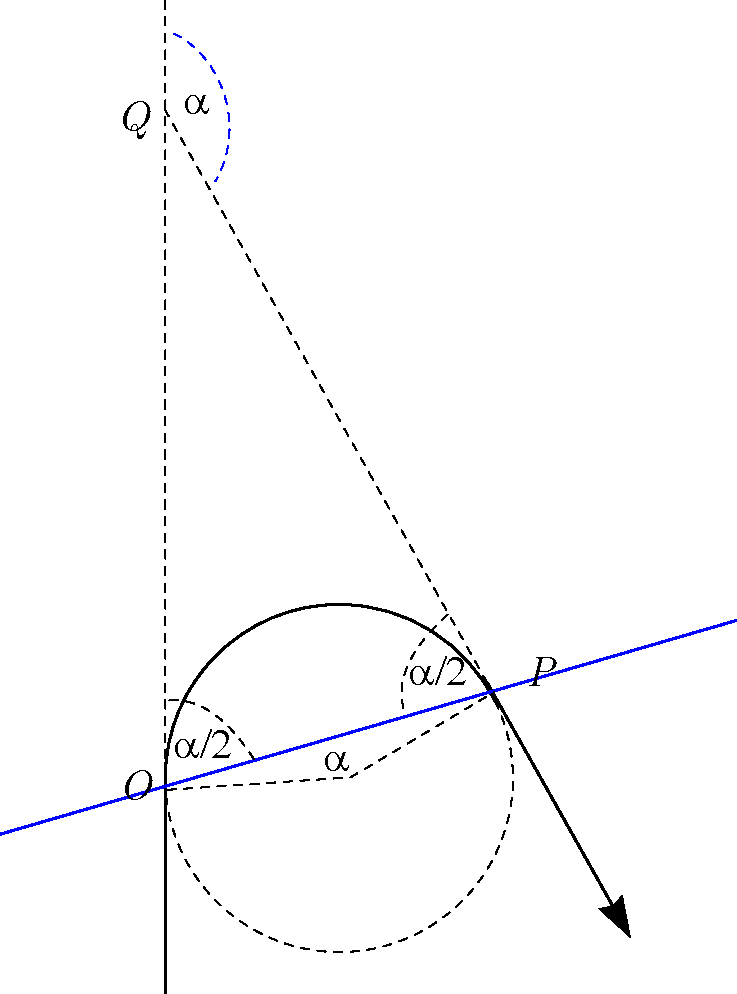
\includegraphics[width = 0.45\textwidth]{2020-v2g-09-yl.pdf}
\end{wrapfigure}



Ruumipiirkonda $y\ge f(x)$ täidab homogeenne $z$-telje sihiline magnetväli tugevusega $B$. Erinevate kiirustega positiivseid ja negatiivseid laenguid kandvad osakesed liiguvad paralleelselt $y$-teljega ja sisenevad magnetväljaga piirkonda punktis $x=y=0$. Magnetväljaga piirkonnast väljudes on kõigi osakeste kiirusvektor pöördunud ühe ja sama nurga $\alpha$ võrra päripäeva, sõltumata laengust, massist ja kiirusest. Visandage osakeste trajektoorid ja leidke funktsioon $f(x)$. 

\hint

\solu
\vspace{-10pt}
  \begin{center}
    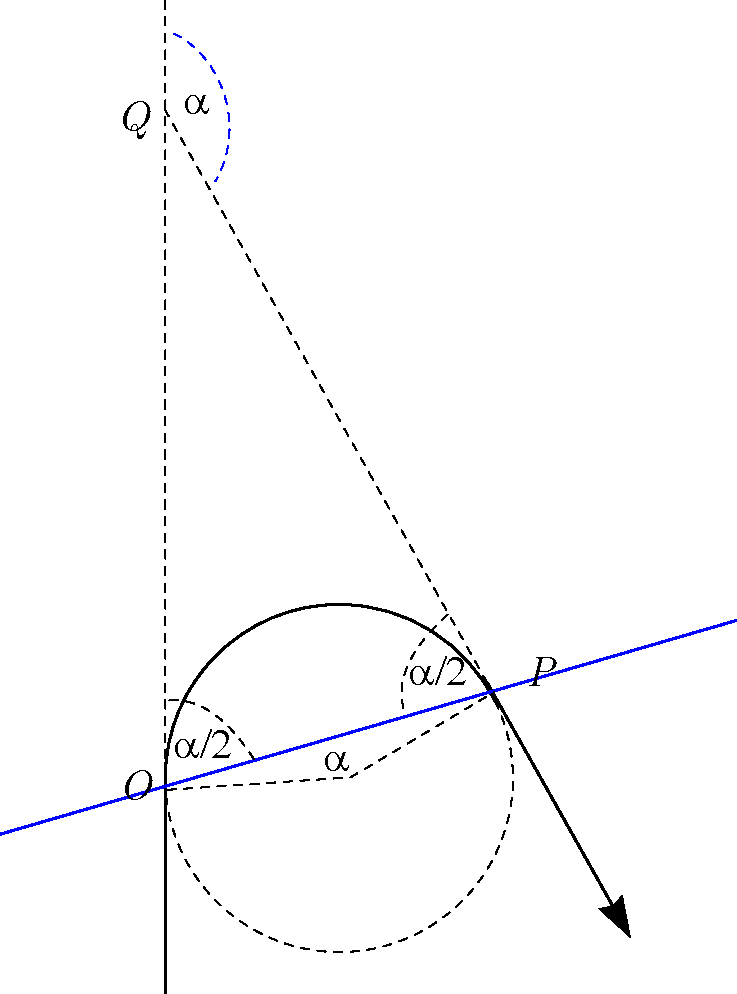
\includegraphics[width=0.5\textwidth]{2020-v2g-09-sol.pdf}
  \end{center}
  \vspace{-10pt}
Lahendus. Sisenegu osake punktis $O$ ja väljugu punktis $P$, kusjuures punkte $O$ ja $P$ ühendab ringjoone kaar --- osakese trajektoor magnetväljas. Lõikugu osakese trajetoori sirgjooneliste lõikude pikendused punktis $Q$, vt joonis. Ülesande tingimuse kohaselt on nurk sirgete $OQ$ ja $QP$ vahel $\alpha$. Et kolmnurk $OQP$ on sümmeetria tõttu võrdhaarne, siis $\angle OQP=\alpha/2$  \pp{3}. Seega peab punkt $P$ asuma sõltumata ringjoone raadiusest sirgel $OP$, mis on $y$-telje suhtes nurga $\alpha/2$ all  \pp{2}, st $f(x)=x\cot(\alpha/2)$  \pp{1}. Punktid joonise eest: on näidatud vähemalt üks trajektoor, millel on kaks sirgjoonelist segmenti, mis on üksteise suhtes nurga $\alpha$ all --- trajektoori osad enne ja pärast magneväljas viibimist --- \pp{2} (kui joonis käsitleb vaid erijuhtu $\alpha=180^\circ$, siis ainult \pp{1}); neid segmente ühendab ringjoone kaare kujuline segment --- \pp{2}; üleminek sirgjooneliselt trajektoorilt ringjooneliseks ja vastupidi on ilma murdekohata (st sirge on ringjoone puutujaks) --- \pp{2}.

\vspace{10pt}
\probend